\documentclass[11pt,a4paper]{article}
\usepackage[top=3cm, bottom=2cm, left=2cm, right=2cm]{geometry}
\usepackage[utf8]{inputenc}
\usepackage{amsmath, amsfonts, amssymb}
\usepackage{siunitx}
\usepackage[brazil]{babel}
\usepackage{graphicx}
\usepackage[margin=10pt,font={small, it},labelfont=bf, textfont=it]{caption}
\usepackage[dvipsnames, svgnames]{xcolor}
\DeclareCaptionFont{MediumOrchid}{\color[svgnames]{MediumOrchid}}
\usepackage[pdftex]{hyperref}
\usepackage{natbib}
\bibliographystyle{plainnat}
\bibpunct{\textcolor{MediumOrchid}{\textbf{[}}}{\textcolor{MediumOrchid}{\textbf{]}}}{,}{s}{}{}
\usepackage{color}
\usepackage{footnote}
\usepackage{setspace}
\usepackage{booktabs}
\usepackage{multirow}
\usepackage{subfigure}
\usepackage{fancyhdr}
\usepackage{leading}
\usepackage{indentfirst}
\usepackage{wrapfig}
\usepackage{mdframed}
\usepackage{etoolbox}
\usepackage[version=4]{mhchem}
\usepackage{enumitem}
\usepackage{caption}
\usepackage{titlesec}
\usepackage{tcolorbox}
\usepackage{tikz}
\usepackage{LobsterTwo}
\usepackage[T1]{fontenc}
\usepackage{fontspec}
\usepackage{txfonts}
\usepackage[bottom]{footmisc}
\tcbuselibrary{skins,breakable}
\sisetup{output-decimal-marker={.}}

\makeatletter
\def\footnoterule{\kern-3pt\color{MediumOrchid}\hrule\@width0.6\textwidth height 0.8pt\kern2.6pt}
\makeatother

\renewcommand{\footnotelayout}{\itshape\color{MediumOrchid}}

\AtBeginEnvironment{equation}{\fontsize{13}{16}\selectfont}


\titleformat{\section}{\LobsterTwo\huge\color{CarnationPink}}{\thesection.}{1em}{}
\titleformat{\subsection}{\LobsterTwo\huge\color{CarnationPink}}{\thesubsection}{1em}{}
\titleformat{\subsubsection}{\bf\LobsterTwo\Large\color{MediumOrchid}}{\thesubsubsection}{1em}{}


\DeclareCaptionLabelFormat{figuras}{\textcolor{DarkTurquoise}{Figura \arabic{figure}}}
\captionsetup[figure]{labelformat=figuras}

\makeatletter
\renewcommand\tagform@[1]{\maketag@@@{\color{CarnationPink}(#1)}}
\makeatother

\renewcommand{\theequation}{Eq. \arabic{equation}}
\renewcommand{\thefigure}{Fig. \arabic{figure}}
\renewcommand{\thesection}{\textcolor{CarnationPink}{\arabic{section}}}

\setlist[itemize]{label=\textcolor{CarnationPink}{$\blacksquare$}}

\setlist[enumerate]{label=\textcolor{CarnationPink}{\arabic*.}, align=left, leftmargin=1.5cm}


\newcounter{exemplo}

\NewDocumentEnvironment{exemplo}{ O{} }{%
\allowbreak
\setlength{\parindent}{0pt}
  \begin{mdframed}[
  leftline=true,
  topline=false,
  rightline=false,
  bottomline=false,
  linewidth=2pt,
  linecolor=CarnationPink,
  frametitlerule=false,
  frametitlefont=\LobsterTwo\large\color{CarnationPink},
  frametitle={\color{CarnationPink}\LobsterTwo\large #1},
  ]
}{%
  \end{mdframed}
}

\setlength{\fboxsep}{5pt}
\setlength{\fboxrule}{1.5pt}
\usepackage{float}
\renewcommand{\thefootnote}{\alph{footnote}}
\usepackage{url}
\hypersetup{
	colorlinks=true,
	linkcolor=DarkTurquoise,
	filecolor=DarkTurquoise,      
	urlcolor=DarkTurquoise,
	citecolor=DarkTurquoise,
	pdftitle={Especialista em Física da Radioterapia}
}
\pagestyle{fancy}
\fancyhf{}
\renewcommand{\headrulewidth}{0pt}
\rfoot{\color{DarkTurquoise}\thepage \\ \LobsterTwo{\small\textcolor{CarnationPink}{@defDalila}}}

\title{\LobsterTwo\Huge{Radioterapia}}
\author{\LobsterTwo\Large{Simulação para o Planejamento do Tratamento}\nocite{*}}
\date{\LobsterTwo\textit{Dalila Mendonça}}
\begin{document}
	\maketitle

\section{Introdução}

	Antes do início da década de 1990, a “simulação” para um tratamento radioterapia consistia apenas em simular o tratamento através de um dispositivo que imitava um acelerador linear (linac) em todos os aspectos, exceto quanto a entrega de um feixe terapêutico. Esses dispositivos (agora chamados de “simuladores convencionais”) são equipados com tubos de raios X de diagnóstico e com equipamentos para formação da imagem e ainda estão em uso. Os simuladores deram lugar em grande parte, no entanto, à simulação através da tomografia computadorizada (TC), em que uma “simulação virtual” é realizada em uma tomografia computadorizada adquirida com o paciente já na posição de tratamento.
	
	A simulação com TC permitiu a era da radioterapia conformacional 3D (3DCRT, no qual os alvos e os tecidos normais são delineados na tomografia computadorizada volumetricamente reconstruída) e para a radioterapia guiada por imagem (IGRT) (que utiliza a tomografia computadorizada como a imagem de referência para o verificação do posicionamento do paciente). Para procedimentos de braquiterapia, as imagens planares ortogonais ainda são amplamente utilizada para localização do aplicador e das estruturas do tecido, embora essa técnica também esteja dando lugar à simulação utilizando imagem volumétrica.

	Os aspectos técnicos dos simuladores de TC e os QA são considerados no TG-66, \textbf{``Quality Assurance for Computed-Tomography Simulators and the Computed-Tomography-Simulation Process''}. Algumas questões específicas a serem consideradas são:

	\begin{itemize}[label=\textcolor{CarnationPink}{$\blacktriangleright$}]
		\item \textcolor{DarkTurquoise}{\textbf{Conversão das Unidades de Hounsfield para Densidade Eletrônica:}} Os valores dos pixels em uma imagem de tomografias computadorizadas estão em unidades Hounsfield (HU), e é necessária uma conversão do número de HU para a sua respectiva densidade eletrônica, que é o parâmetro com respeito ao meio que os cálculos de dose exigem. A conversão é realizada com um phantom para calibração e são necessárias verificações anuais dessa conversão.
		
		\item \textcolor{DarkTurquoise}{\textbf{Artefatos Metálicos:}} Ees podem obscurecer as estruturas do tecido e resultar na imprecisão nos cálculos de dose. Como por exemplo os artefatos dentários em imagens de cabeça e pescoço ou uma prótese de quadril para tratamentos da pelve (ver, por exemplo, AAPM TG-63, \textcolor{MediumOrchid}{\textit{\textbf{``Dosimetric considerations for patients with hip prostheses undergoing pelvic irradiation''}}}). A densidade dos artefatos de metal pode precisar ser substituída no sistema de planejamento de tratamento. Algoritmos para redução de artefatos de metal estão agora disponíveis em alguns tomógrafos. Problemas com os artefatos de TC também podem ser evitados utilizando configurações clínicas apropriadas para alguns tratamentos ou usando TC de megavoltagem (por exemplo, TomoTherapy).
		
		\item \textcolor{DarkTurquoise}{\textbf{Equipamentos de TC com Bore Largo:}} Como muitas vezes é necessário acomodar os pacientes na posição de tratamento (por exemplo, em uma prancha inclinada), os scanners com um diâmetro grande do bore são os mais indicados. Os modelos disponíveis incluem o Brilliance CT Big Bore (Philips Inc., Eindhoven, Holanda) com diâmetro do bore de 85 cm, o Somatom (Siemens Inc., Ehrlangen, Alemanha) com diâmetro do bore de 80 cm e o Airo intraoperatório CT com diâmetro do bore de 107 cm (Brainlab Inc., Feldkirchen, Alemanha). Além do tamanho do bore, o tamanho do campo de visão (FOV) também é importante. Se o scanner tiver um grande bore, mas um FOV padrão, o paciente e os dispositivos podem passar pelo bore, mas a superfície da pele pode não ser visualizada, tornando a varredura inútil. Alguns scanners podem reconstruir com FOVs maiores, mas estes devem ser verificados cuidadosamente com respeito à HU e a precisão geométrica.
	\end{itemize}

	A ressonância magnética (MRI) e a tomografia por emissão de pósitrons (PET)/CT estão sendo cada vez mais aplicadas no planejamento do tratamento de Radioterapia. Se o objetivo é utilizar esses estudos para definir os volumes-alvo, a posição do paciente no scanner da ressonância magnética ou no PET/TC deve corresponder o mais próximo possível da posição de tratamento (por exemplo, mesa plana, mesmos acessórios de imobilização e mesmo posicionamento). Atualmente, existem acessórios de imobilização compatíveis com MRI disponíveis pelos fornecedores. Um desafio é que normalmente os exames de ressonância magnética ou PET/TC realizados para estadiamento são adquiridos antes mesmo da simulação de radioterapia ser realizada, o que dificulta a utilização dos acessórios compatíveis com RMI nessas aquisições. O uso da ressonância magnética para simulação provavelmente será um tópico importante à medida que os dispositivos de tratamento habilitados para ressonância magnética se tornarem cada vez mais amplamente utilizados.

\section{Imobilização, Setup e Marcação dos Pacientes}

	No geral, o objetivo de estabelecer um setup para o paciente é \textit{\textcolor{MediumOrchid}{(i)}} reduzir a movimentação do paciente, \textit{\textcolor{MediumOrchid}{(ii)}} tornar o posicionamento diário mais reprodutível, \textit{\textcolor{MediumOrchid}{(iii)}}  melhorar o conforto do paciente e \textit{\textcolor{MediumOrchid}{(iv)}} otimizar a prevenção dos tecidos normais.

	Reduzir a amplitude da movimentação é especialmente importante devido ao fato de que os pacientes geralmente ficam na mesa de tratamento por aproximadamente 15 minutos ou mais, principalmente para tratamentos de radiocirurgia estereotáxica (SRS)/ ou estereotaxia extra-craniana (SBRT), que além de ficar um longo período na sala, ainda é entregue uma alta dose por fração. 
	
	Os mesmos acessórios de imobilização devem ser utilizados tanto para a simulação quanto para o tratamento. Algumas opções de acessórios de imobilização incluem apoios de cabeça especializados, rampas inclinadas e suportes de braço para pacientes com mama e “\textit{belly boards - pranchas de barriga}”  para alguns tratamentos abdominais em decúbito ventral. Um acessório amplamente utilizado é a máscara termoplástica, que normalmente consiste de um plástico perfurado que amolece quando aquecido e enrijece a medida que vai se esfriando. 
	
	Os materiais termoplásticos estão disponíveis em diferentes espessuras, com materiais mais espessos oferecendo maior rigidez ao custo de uma menor preservação da pele. Os materiais termoplásticos mais espessos podem dobrar ou até triplicar a dose na pele, conforme descrito no AAPM TG-176, \textit{\textbf{``Dosimetric Effects Caused by Couch Tops and Immobilization Devices''}}. Para pacientes levemente claustrofóbicos, cortar a máscara na região dos olhos e, se necessário, na região da boca pode aumentar o conforto do paciente de forma suficiente para evitar a necessidade de sedação. Vários fabricantes já estão oferecendo máscaras pré-cortadas para esta finalidade.

	Para promover uma melhor segurança, a maioria dos dispositivos de imobilização modernos podem ser “indexados” – ou seja, fixados à mesa de tratamento em locais claramente e precisamente definidos. Como a posição do paciente é fixa em relação à mesa de tratamento, as coordenadas X, Y e Z da mesa podem ser verificadas diariamente quanto à sua consistência.

\subsection*{Marcação dos Pacientes}

	Uma configuração de três pontos é comumente utilizada para alinhar os pacientes. Com essa técnica, três retículos de lasers são visualizados na pele: dois pontos laterais (um de cada lado) e um ponto anterior (supondo que o paciente esteja em decúbito dorsal). Conceitualmente, a configuração de três pontos determina a localização do isocentro e auxilia no controle da a rotação (roll) do paciente (a inclinação pitch e a guinada yall são um pouco menos restritas). 

	Às vezes, marcas extras na pele podem ser utilizadas para auxiliar o posicionamento, melhorando o alinhamento do paciente. Por exemplo, um conjunto de “marcas de nivelamento” colocadas inferiormente pode ser utilizada para posicionar um paciente com câncer de mama porque a mobilidade do tecido mamário torna as marcas na região da mama menos adequadas para o alinhamento. Antes da tomografia computadorizada, um ``ball bearing'' (BB) é normalmente colocado em cada uma das 3 marcas de setup (origem) para que o ponto de intersecção das coordenadas possam ser visualizados na tomografia computadorizada. Marcadores alternativos estão disponíveis, como o retículo de plástico CT-SPOT (Beekley Medical Inc., Bristol, CT).
	
	Em algumas instituições o paciente pode receber uma pequena tatuagem feita com tinta permanente em cada um dos pontos finais que determinam o isocentro do tratamento. Em alguns casos, no entanto, o isocentro final pode não ser determinado no momento da simulação, e então é deixada uma marca temporária no paciente. As mudanças necessárias das marcas de origem para as marcas de tratamento são então determinadas no sistema de planejamento de tratamento e, em seguida, as tatuagens finais são feitas no paciente (por exemplo, no primeiro dia de imagem).
	
	Para verificar a posição correta do paciente e/ou do campo de tratamento, as radiografias (“filmes de portal”) são frequentemente utilizadas na máquina de tratamento. Essas imagens são comparadas com radiografias reconstruídas digitalmente (DRRs) geradas a partir da CT de simulação.

	Outras marcações/marcadores às vezes são utilizados no momento das simulações para diversas finalidades. Para pacientes que recebem o tratamento adjuvante, por exemplo, a cicatriz cirúrgica pode ser marcada para ser uma referência na elaboração do plano de tratamento (as cicatrizes são um local de recorrência em alguns casos sendo necessário um boost nessa região em muitas das vezes). Um “fio” de plástico radiopaco é normalmente utilizado para essa finalidade. O fio de metal é muitas das vezes evitado porque produz artefatos na tomografia computadorizada. Em casos pós-operatórios também é comum marcar o local do dreno cirúrgico com fio ou BB. Os fios às vezes são utilizados para marcar a extensão do tecido mamário palpável, por exemplo. Como exemplo final, os marcadores costumam ser utilizados para indicar a lateralidade e ajudar a garantir que o local de tratamento correto seja identificado na imagem. Um exemplo disso é a radiocirurgia estereotáxica para neuralgia do trigêmeo. Um BB é colocado na cabeça do paciente no lado envolvido, o que ajuda a garantir que o quinto nervo craniano correto seja identificado.

	Existem várias pontos falhos relacionadas ao setup e às marcações de referência:

	\begin{enumerate}[label=\textcolor{CarnationPink}{(\arabic*)}]
		\item Se o ponto do isocentro for movido no sistema de planejamento em relação ao ponto de origem definido na tomografia de simulação, fornecendo um deslocamento, isso poderá resultar em um setup incorreto do paciente, a menos que o deslocamento seja claramente comunicada a toda a equipe de tratamento.
		\item Deve-se tomar cuidado ao identificar o BB correto para definir o ponto de origem nas imagens de TC. Pode ocorrer uma certa confusão caso BBs extras ou outros fiduciais estiverem sendo utilizados para marcações de outros elementos importantes (por exemplo, um BB em um local de drenagem ou fio de plástico em uma cicatriz cirúrgica).
		\item Se um paciente receber uma re-irradiação em uma área semelhante, deve-se tomar cuidado para não confundir a tatuagem antiga com o isocentro do novo local pretendido. Uma boa comunicação é essencial.
		\item Pintas ou sardas às vezes podem ser confundidas com tatuagens. Fotos e documentação podem ajudar a evitar problemas desta natureza.
	\end{enumerate}

\subsection*{Bolus}

	Um bolus feito com um material tecido-equivalente pode ser adicionado aos feixes de fótons ou elétrons com a finalidade de aumentar a dose superficial. Embora o bolus possa ser adicionado digitalmente no sistema de planejamento de tratamento, às vezes é vantajoso colocar o material do bolus real no momento da tomografia de simulação para determinar com precisão sua posição, sua forma e seu efeito dosimétrico. O bolus tecido-equivalente pode assumir uma variedade de formas (\ref{fig:bolus}), incluindo:

	\begin{itemize}[label=\textcolor{CarnationPink}{$\blacksquare$}]
		\item \textcolor{DarkTurquoise}{\textbf{Folhas de gel como Superflab ou Elastogel:}} São fáceis de usar e a espessura é bem definida, mas podem não se adaptar bem a superfícies curvas.
		
		\item \textcolor{DarkTurquoise}{\textbf{Materiais maleáveis, como pastilhas termoplásticas, cera de abelha ou parafina:}} Útil para superfícies altamente curvas e particularmente para tratamentos com feixes de elétrons. Para tratamentos com elétrons, o material do bolus pode ser moldado em formas de modo a preencher as cavidades de ar, como a cavidade nasal.
		
		\item \textcolor{DarkTurquoise}{\textbf{Superstuff:}} Como a cera, esse material pode ser moldado para adaptar a diferentes formas.
		
		\item \textcolor{DarkTurquoise}{\textbf{Gaze ou toalhas molhadas:}} Estes são úteis para superfícies curvas, mas a gaze deve ser consistentemente saturada com água para atingir o efeito bolus (dosimétrico) pretendido.
		
		\item \textcolor{DarkTurquoise}{\textbf{Brass metal mesh\cite{healy2013skin}, beam spoiler e Vaselina espessa:}} Estes são todos úteis para tratamentos de câncer de mama.
	\end{itemize}

	\begin{figure}[h]
		\centering
		\subfigure[Elastogel]{
			\fcolorbox{DarkTurquoise}{white}{%
				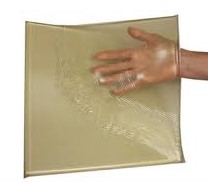
\includegraphics[width=0.19\textwidth]{Imagens/bolusgel.jpg}
			}} %
			\subfigure[Superflab]{
		\fcolorbox{DarkTurquoise}{white}{%
			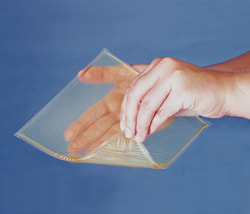
\includegraphics[width=0.19\textwidth]{Imagens/estogel.jpg}
		}} % 
		\subfigure[Brass metal mesh]{
			\fcolorbox{DarkTurquoise}{white}{%
				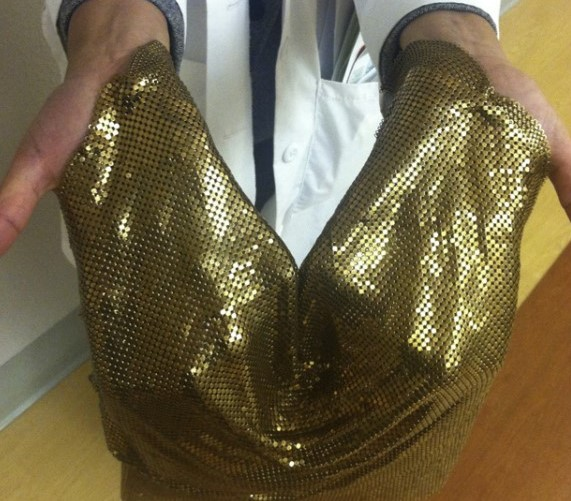
\includegraphics[width=0.19\textwidth]{Imagens/bressMesh.jpg}
			}}  %
			\subfigure[Brass metal mesh]{
		\fcolorbox{DarkTurquoise}{white}{%
			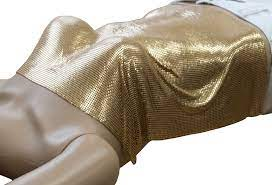
\includegraphics[width=0.24\textwidth]{Imagens/bressMessh2.jpg}
		}} \\ % 
		\subfigure[Superstuff]{
			\fcolorbox{DarkTurquoise}{white}{%
				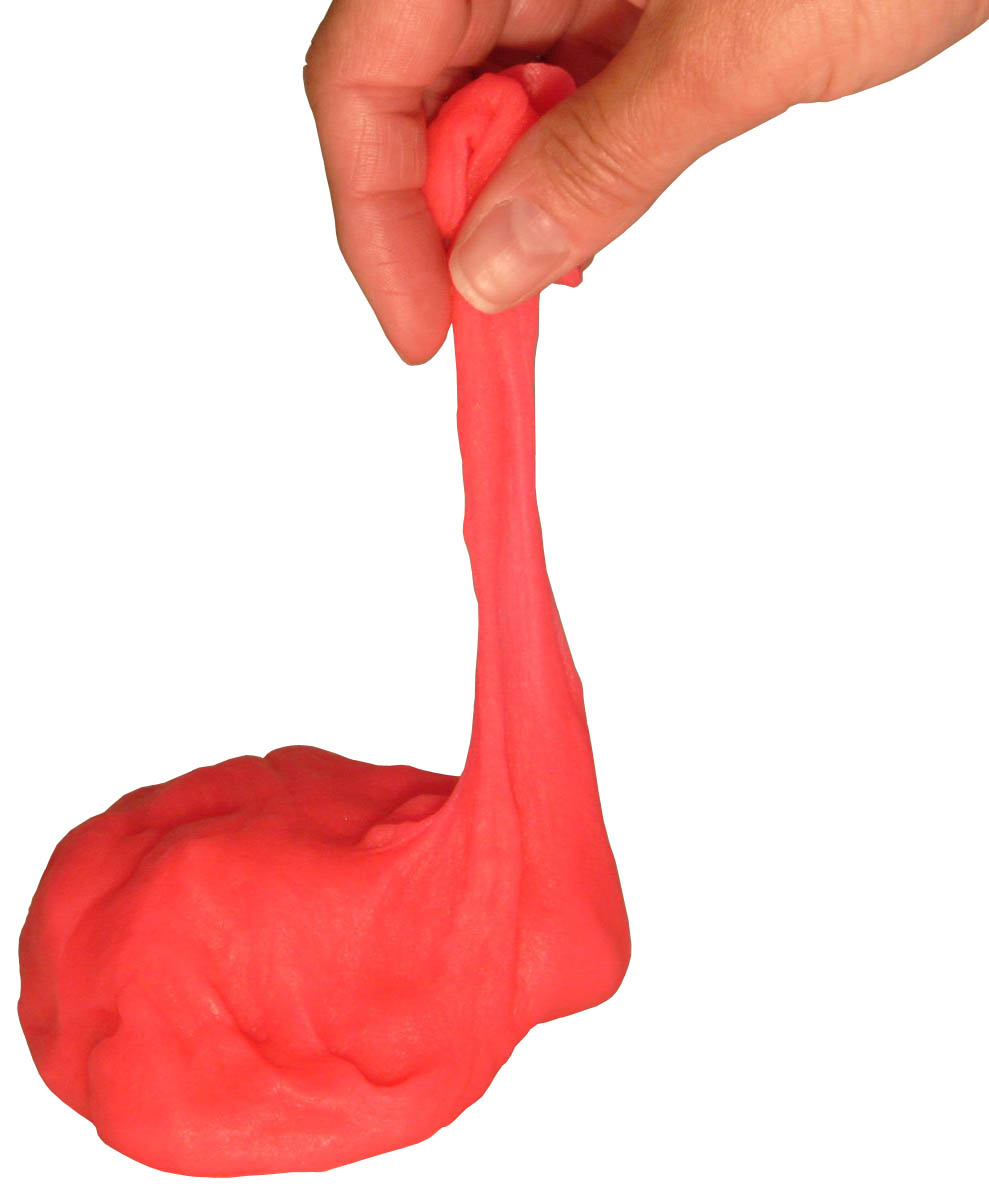
\includegraphics[width=0.14\textwidth]{Imagens/SuperStuffBolus.jpg}
			}} %
			\subfigure[Superstuff]{
		\fcolorbox{DarkTurquoise}{white}{%
			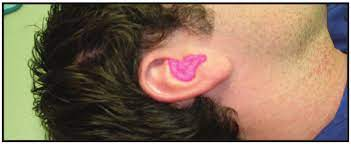
\includegraphics[width=0.42\textwidth]{Imagens/superstuff.jpg}
		}}  % 
			\subfigure[Parafina]{
		\fcolorbox{DarkTurquoise}{white}{%
			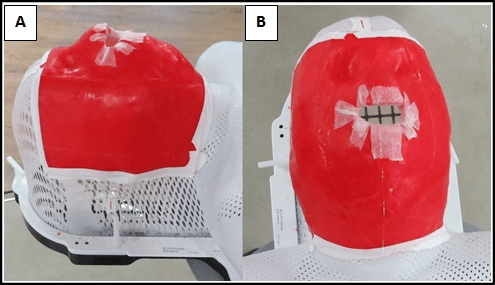
\includegraphics[width=0.3\textwidth]{Imagens/parafina.png}
		}} \\ % 
		\subfigure[Termoplastic Pellets]{
			\fcolorbox{DarkTurquoise}{white}{%
				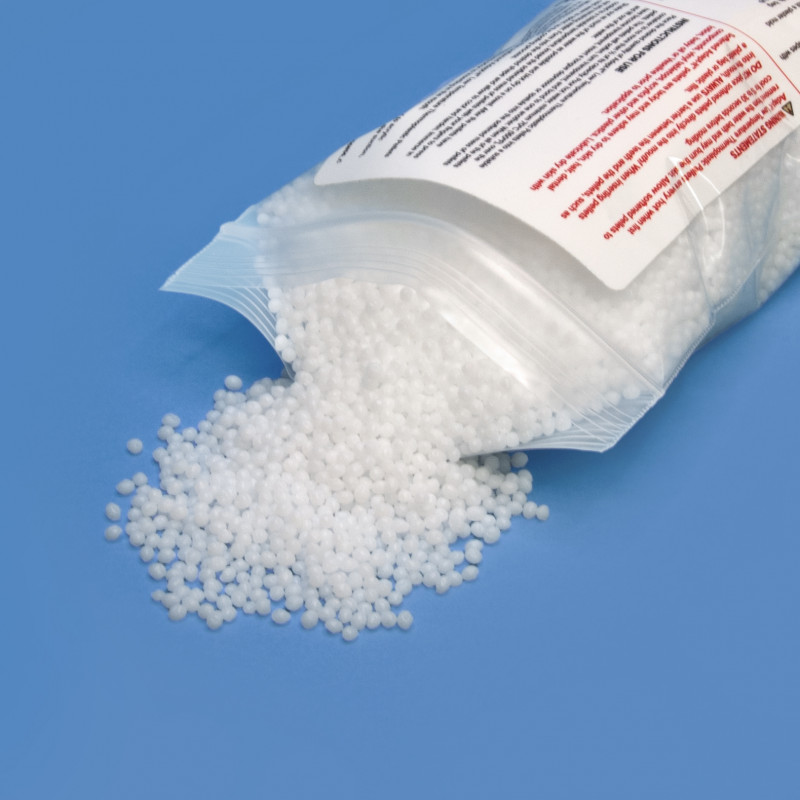
\includegraphics[width=0.15\textwidth]{Imagens/termoplasticpellets.jpg}
			}} %
			\subfigure[Termoplastic]{
		\fcolorbox{DarkTurquoise}{white}{%
			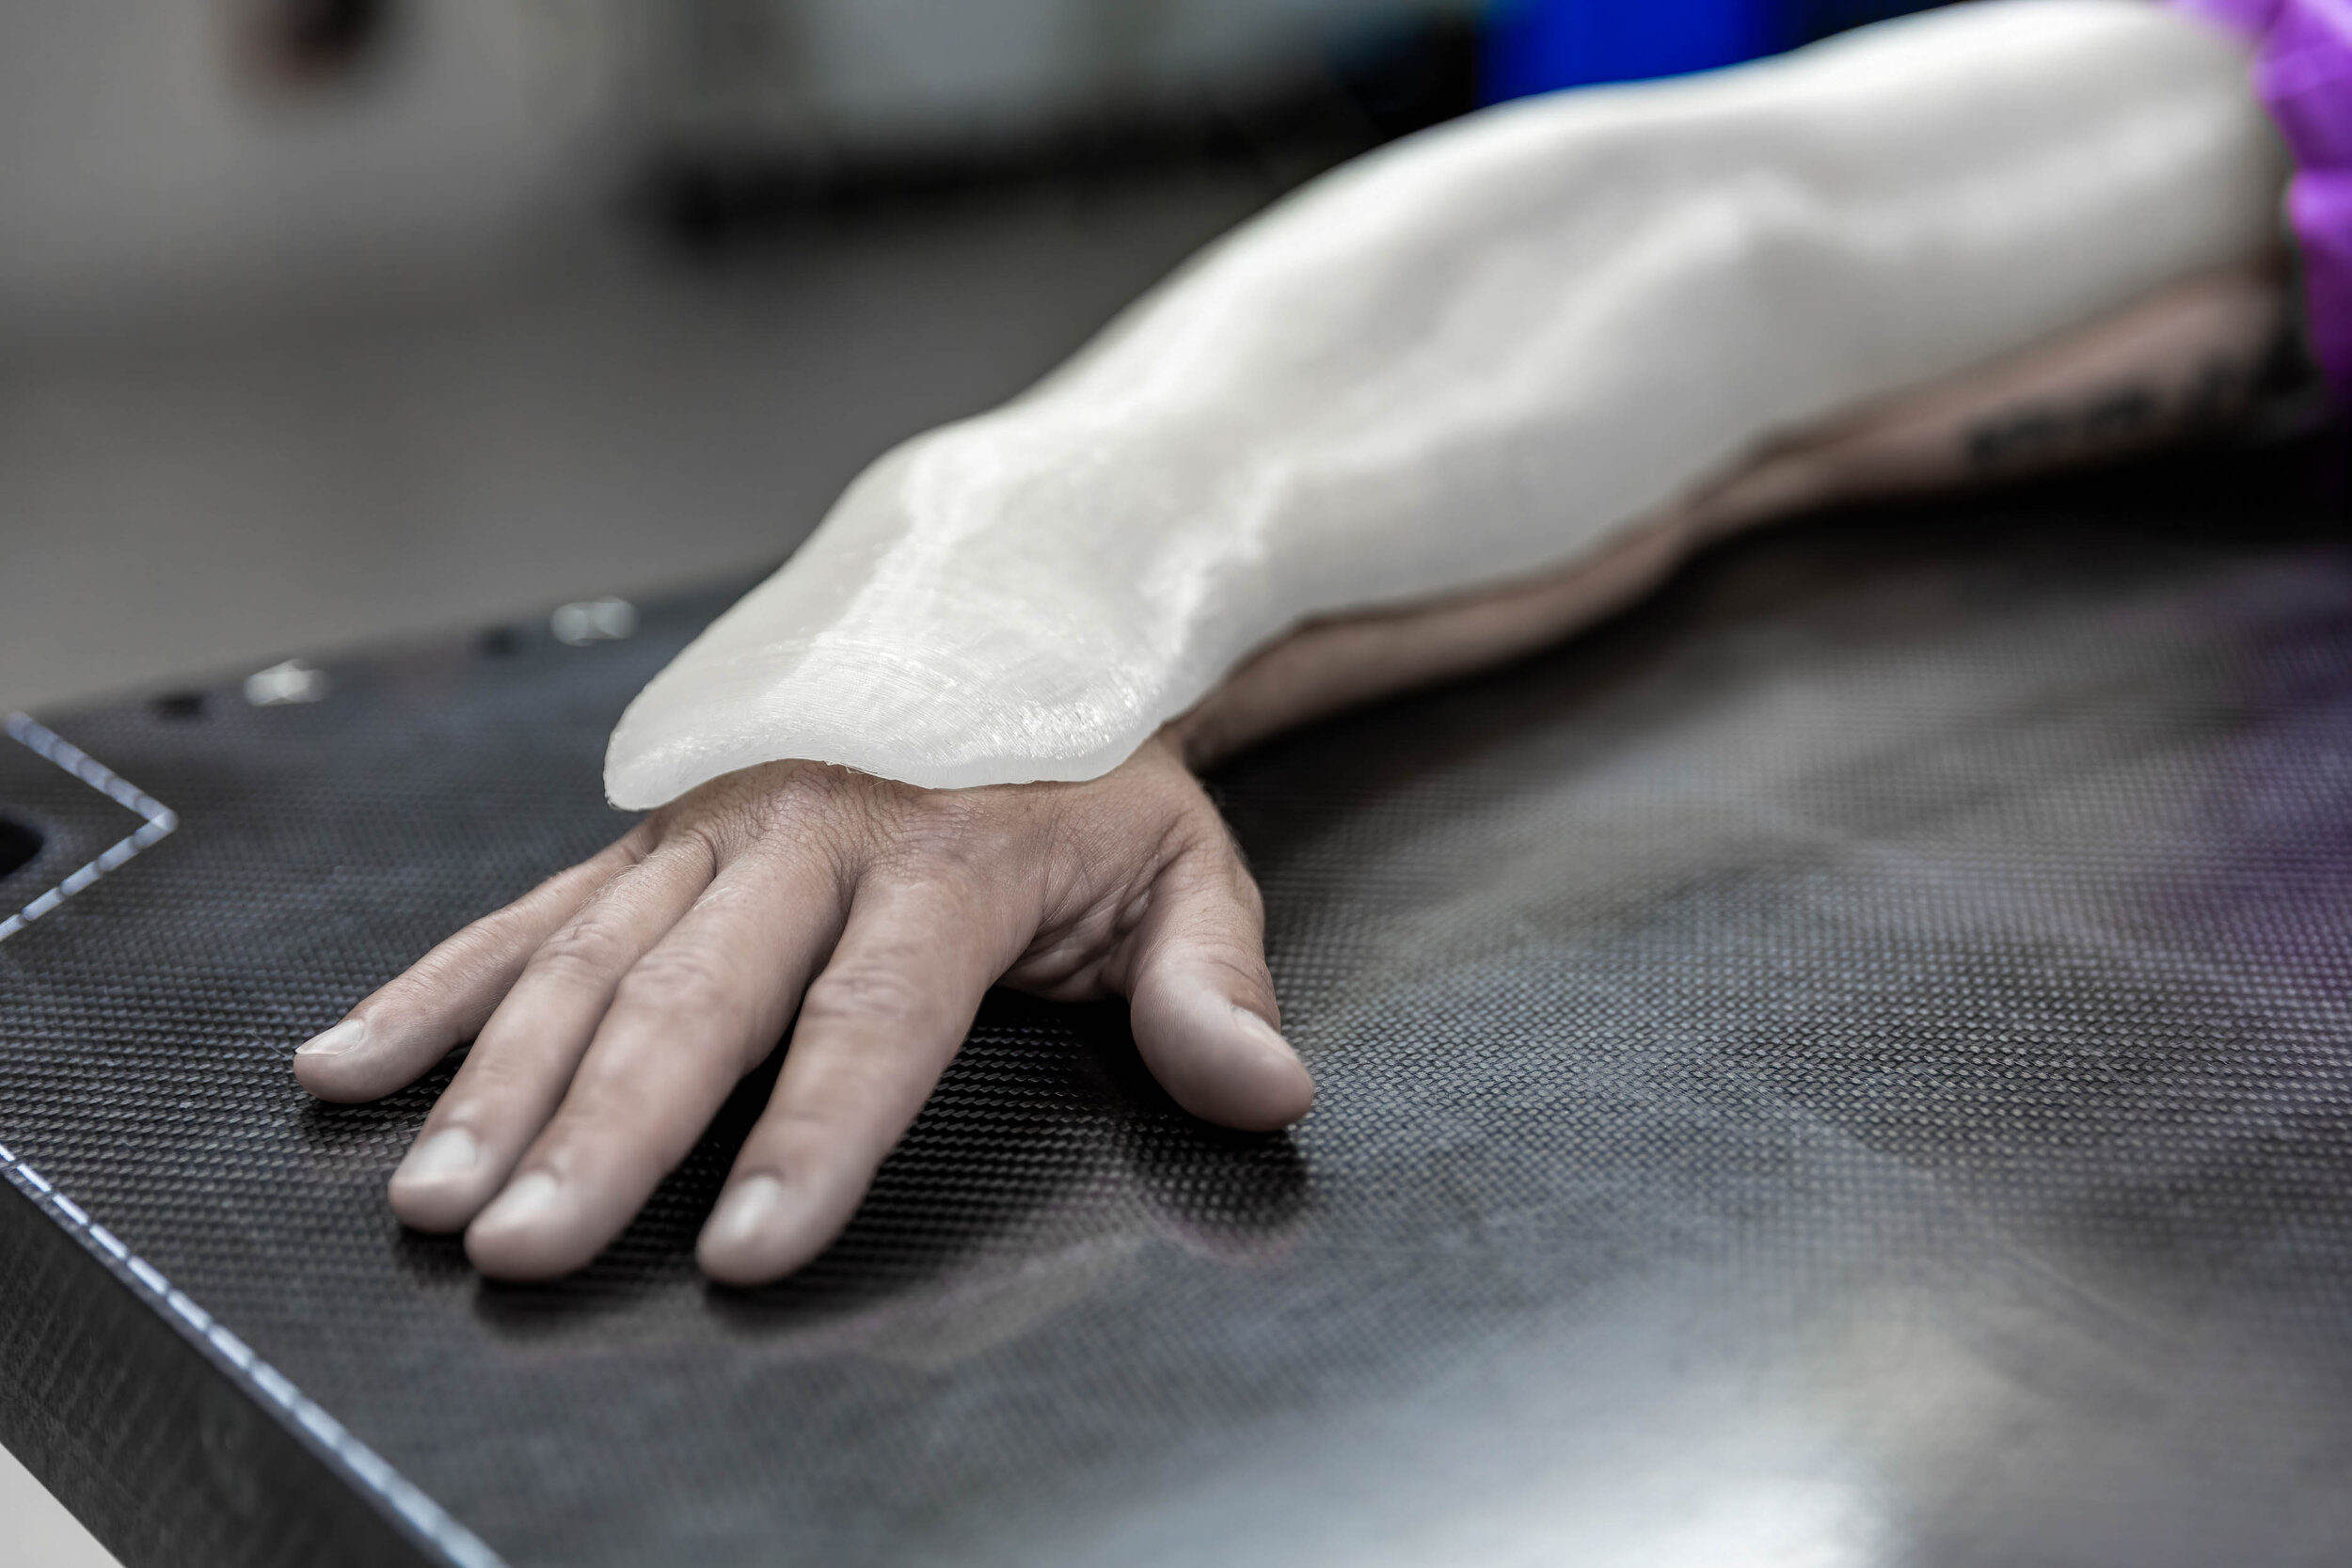
\includegraphics[width=0.22\textwidth]{Imagens/termoplstic.jpg}
		}}  %
		\subfigure[Beam Spoiler]{
			\fcolorbox{DarkTurquoise}{white}{%
				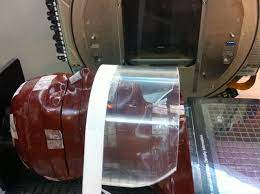
\includegraphics[width=0.2\textwidth]{Imagens/beamspoiler1.jpg}
			}} %
			\subfigure[Beam Spoiler]{
		\fcolorbox{DarkTurquoise}{white}{%
			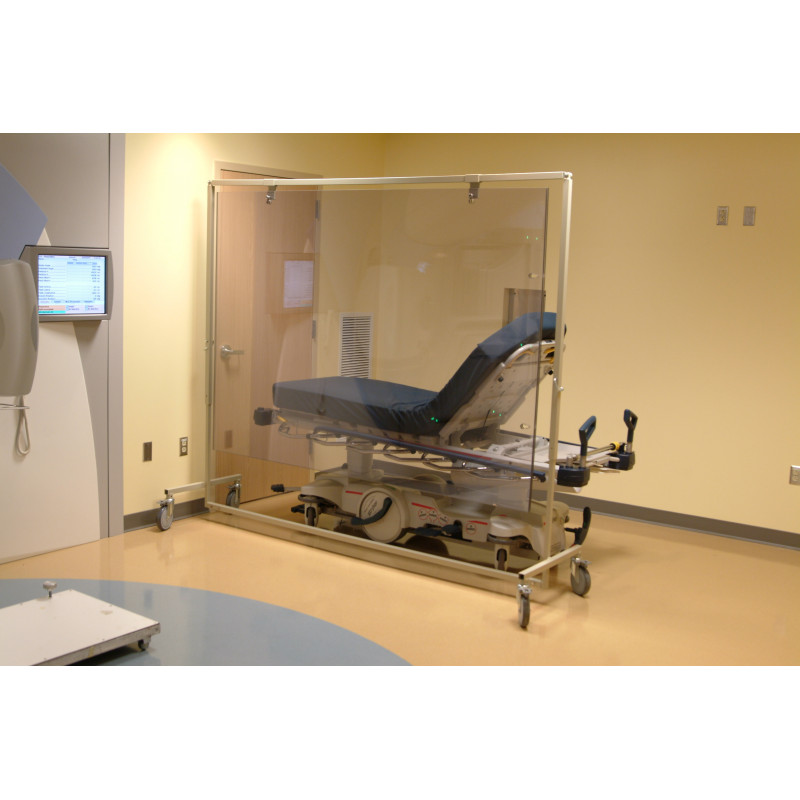
\includegraphics[width=0.15\textwidth]{Imagens/beamspoiler2.jpg}
		}}  %
		\caption{Exemplos de Bolus}
		\label{fig:bolus}
	\end{figure}

	Qualquer que seja o material de bolus utilizado, deve-se tomar cuidado para garantir que o material fique plano diretamente em contato com a pele evitando gaps de ar. Grandes gaps de ar produzem um espalhamento lateral dos elétrons, o que pode levar a uma dose reduzida na borda distal da cavidade e até mesmo a uma segunda região de buildup. Este efeito é maior para tamanhos de campo pequenos, grandes gaps de ar e para energias mais altas. O efeito dos gaps de ar foram estudados, mas a maioria dos reports se concentram na precisão dos algoritmos de planejamento para prever a dose além desses gaps de ar. No entanto, estudos realizados em tratamentos de cabeça e pescoço sugeriram que o efeito das cavidades de ar é da ordem de 2\% para grandes tamanhos de campo. Para gaps de ar menores que aproximadamente 1 cm, o impacto não parece ser clinicamente significativo.

\subsection*{Blindagens}

	As blindagens de radiação são frequentemente construídas ou testadas no momento da simulação. Alguns exemplos de blindagens são:

	\begin{itemize}[label=\textcolor{CarnationPink}{$\blacksquare$}]
		\item \textcolor{DarkTurquoise}{\textbf{Protetores oculares usados para proteger o cristalino e a córnea durante tratamentos da pálpebra com elétrons:}} Dispositivos comercialmente disponíveis especificamente projetados para tratamentos com feixes de elétrons de alta energia. Um exemplo de produto é uma blindagem de tungstênio curva de 2 a 3 mm de espessura coberta com acrílico para evitar os elétrons retroespalhados. Uma blindagem de 2 a 3 mm resulta em uma transmissão de aproximadamente 4\%.		

		\item \textcolor{DarkTurquoise}{\textbf{Blindagens de chumbo colocadas na superfície da pele para tratamentos com elétrons:}} O objetivo principal é criar uma penumbra mais nítida na borda do campo. A blindagem deve ser espessa o suficiente para atenuar o feixe. Uma regra prática típica é, a espessura do chumbo (mm) = Energia (em MV)/2 + 1. Deve ser feita uma blindagem 20\% mais espessa caso o material utilizado para confecção da blindagem for o cerrobend.		
		
		\item \textcolor{DarkTurquoise}{\textbf{Escudo testicular ou “clamshell- concha”:}} Estas blindagens são normalmente construídas com chumbo de 1.25 cm de espessura com uma fenda para acesso, projetada de forma a evitar que a radiação espalhada atinja os testículos. As Clamshells podem ser úteis em uma variedade de aplicações porque a aspermia permanente ocorre como resultado de exposição a doses $>$ 2 Gy. Dados do SWOG-8711 apoiam o uso de tais blindagens no tratamento de câncer testicular.
	\end{itemize}

\section{Simulação com TC}

	Antes do exame, a paciente deve ser avaliada quanto ao estado de gravidez, os pacientes devem ser avaliados quanto a presença de dispositivos cardíacos ou outros dispositivos eletrônicos implantados e quanto a possíveis contraindicações para o uso de contraste. Além disso, o paciente deve ter sido treinado em relação ao preparo com respeito ao preenchimento retal e/ou da bexiga, quando relevante. O médico também deve ter especificado os objetivos da simulação e dado claramente as orientações quanto aos requisitos técnicos da simulação por exemplo, dispositivos de imobilização, controle respiratório e a extensão anatômica necessária na aquisição da imagem.

	Depois que o setup e a imobilização estiverem concluídos, a primeira etapa geralmente é alinhar o paciente com base em uma imagem de referência ântero-posterior chamada de “scout”. Isso ajuda em um posterior alinhamento porque quanto mais reto o paciente estiver mais fácil é reproduzir seu posicionamento. Uma exceção é para aqueles pacientes que, por razões ou limitações médicas, se sentem mais confortáveis em uma posição levemente curvada. Observou-se que forçar esses pacientes a um alinhamento reto pode causar problemas de reprodutibilidade durante o tratamento.É importante notar que as imagens de scout normalmente não são dimensionalmente corretas no aspecto lateral devido à divergência do feixe leque. 
	
	Os pacientes geralmente são posicionados em decúbito dorsal, mas outras posições fora do padrão são possíveis (por exemplo, supino com os pés para o gantry para o tratamento de uma lesão na perna, decúbito ventral para um paciente em um belly board ou mesmo decúbito para outras aplicações). O posicionamento deve ser anotado corretamente no console do tomógrafo para que ele preencha corretamente o cabeçalho do arquivo DICOM (quem me dera). A falha em observar corretamente o posicionamento pode resultar em problemas de orientação durante o planejamento do tratamento ou durante as sessões de radioterapia guiada por imagem (IGRT).

	Os agentes de contraste são frequentemente utilizados durante a simulação para melhorar a visualização de algumas estruturas. Esses agentes têm números de HU altos devido ao seu alto número atômico. Uma formulação de contraste é o sulfato de bário líquido que é engolido para visualizar o trato gastrointestinal inferior (GI) ou ingerido como uma pasta para visualizar o trato GI superior e o esôfago.
	
	Agentes de contraste iodados são injetados por via intravenosa (IV) para destacar a vasculatura e/ou tumores. O momento da injeção IV pode ser correlacionado com a varredura para destacar as artérias (na fase inicial da disseminação do contraste) ou as veias (na fase tardia do contraste). Os tumores também são visualizados de forma diferente nessas várias fases de uma forma dependente da histologia. O tempo da injeção IV geralmente é coordenado por meio de uma bomba injetora que administra o contraste remotamente, por meio de um cateter feito de plástico com um calibre de 20 ou superior.
	
	Informações detalhadas sobre as técnicas de contraste e as considerações médicas podem ser encontradas no Manual sobre meios de contraste do American College of Radiology (ACR). Em teoria, a presença de um agente de contraste pode afetar os cálculos da dose, uma vez que o algoritmo enxerga o contraste como um “osso” de alta densidade para os cálculos de dose. Alguns estudos avaliaram este cenário, no entanto, concluíram que o efeito é pequeno.
	
	O agente de contraste também pode causar problemas na fusão entre imagens. Por exemplo, utilizar o contraste de bário em pacientes que recebem tratamento com rastreamento da coluna no CyberKnife pode impedir que o algoritmo de imagem funcione corretamente. Problemas semelhantes estão começando a aparecer à medida que os algoritmos de setup guiados por imagem utilizandos em linacs são utilizados. Para resolver esses problemas, é possível adquirir primeiro uma varredura sem contraste e utilizá-la para os cálculos de dose e para a orientação por imagem, enquanto a varredura com contraste é utilizada como um conjunto de imagens de fusão para melhor visualização.

	Durante a tomografia computadorizada, o FOV deve ser configurado para que toda a superfície do paciente esteja incluída nas imagens de TC. Embora varreduras com pequenos FOV possam ser aceitáveis ou até mesmo desejáveis para análises na radiologia diagnóstica, o contorno externo do paciente é necessário para fins de planejamento de tratamento e para o alinhamento de algumas técnicas de IGRT.
	
	Pacientes obesos representam um desafio, pois o FOV pode não ser suficiente para englobar todo o paciente. Para lesões lateralizadas em pacientes obesos, o paciente pode ser deslocado para o lado contralateral à lesão na mesa de TC para adquirir o máximo possível da superfície ipsilateral à lesão. Também pode ocorrer perda tecidual se um paciente estiver posicionado longe do eixo central da varredura. Nessas situações, a tomografia computadorizada pode ser modificada para incorporar uma estimativa dos tecidos ausentes, que podem ser derivados de medidas de separação (DAP ou DLL).

	A medida e o monitoramento do movimento respiratório são outros aspectos importantes a serem avaliados na simulação. O movimento respiratório pode ser mensurado com uma TC 4D ou através de imagens de fluoroscopia, conforme descrito no AAPM TG-76, \textit{\textbf{``The Management of Respiratory Motion in Radiation Oncology''}}. Políticas e procedimentos devem estar bem estabelecidos para situações em que podem ser necessários múltiplos exames de TC 4D, uma vez que a dose é substancialmente maior para tais aquisições. É importante lembrar que o movimento respiratório afeta não apenas o pulmão, mas também o abdome; Grandes movimentações foram medidas para o fígado e para os rins.
	
	O movimento respiratório pode ser controlado por vários meios, incluindo compressão abdominal, controle respiratório (respiratory gating) e retenção da respiração (breath hold). Qualquer que seja a solução empregada para o monitoramento respiratório, esse mesmo sistema (com as mesmas configurações) deve ser utilizado tanto na simulação quanto no tratamento. 

	Uma consideração final com respeito a TC de simulação é a exposição recebida pelo paciente. Embora as doses da imagem sejam muito menores do que as doses terapêuticas que o paciente receberá, o AAPM TG-75, \textbf{\textit{``The Management of Imaging Dose During Image-Guided Radiotherapy''}}, sugere que a dose administrada pelas imagens deve ser considerada e minimizada sempre que possível. O monitoramento da dose da TC agora está sendo amplamente utilizado na radiologia com vários produtos comerciais disponíveis, bem como um registro ACR. Alguns departamentos de Radioterapia também estão adotando a prática, e isso pode se tornar uma prática padrão.

\section{Captura de Superfície Utilizando Rastreamento Ótico}

	Um dos sistemam de IGRT depende do alinhamento e/ou o rastreamento (tracking) da superfície de um paciente. Uma das tecnologias utilizadas para este fim é através da projeção e detecção de de padrões de luz mapeados na superfície do paciente (por exemplo, AlignRT, VisionRT Ltd., Londres, Reino Unido). Outra tecnologia utiliza lasers de varredura 3D para obter imagens da superfície do paciente (por exemplo, Sentinel, C-Rad, Uppsala, Suécia).
	
	Essas tecnologias podem utilizar a própria imagem de TC de planejamento como imagem de referência, ou pode utilizar uma imagem óptica como referência, que  pode ser obtida no momento da simulação para posterior comparação. Os guidelines de QA são encontrados no AAPM TG-147, \textit{\textbf{``Quality Assurance for Nonradiographic Radiotherapy Localization and 	Positioning Systems''}}.

\section{Processamento Pós-Aquisição}

	Após a aquisição da imagem de simulação, deve ser realizado um controle de qualidade. Este QA pode incluir uma verificação do preparo do reto ou da bexiga para os sítios de tratamento que estas análises são significativas. Este QA também inclui uma verificação dos dados demográficos e da orientação do paciente e a importação desses parâmetros e das imagens para o sistema de planejamento. Se é preciso realizar uma fusão de imagens (por exemplo, MRI ou PET), a qualidade da fusão também deve ser conferida.

	Às vezes, é levantada a questão quanto à necessidade das tomografias computadorizadas adquiridas para fins de planejamento de radioterapia serem formalmente avaliadas por um radiologista. Um estudo recente examina a incidência de achados incidentais e  resume varios outros estudos que avaliaram essa questão. Os autores concluem que, embora a taxa de achados incidentais possa ser substancial (até 20\%), a abordagem definida para o tratamento é alterada em apenas $\sim$1\% dos casos.

	Uma questão relacionada é com respeito as imagens adquiridas para Radioterapia, para definir se é necessário transferi-las para o sistema de comunicação e arquivamento de imagens radiológicas (PACS), quando disponível. Essa é uma boa prática, pois outro médico pode encontrar as imagens no PACS, que é um meio eficiente de arquivamento de dados.

\section{Considerações Relacionadas à Segurança Clínica}

\subsection*{Utilização de Agentes de Contraste}

	As diretrizes práticas do American College of Radiology (ACR) e Society for Pediatric Radiology (SPR) descrevem as recomendações gerais para o uso de contraste juntamente com as políticas, os procedimentos e a documentação associada a esta prátiva. Uma consideração detalhada das questões clínicas relacionadas aos meios de contraste pode ser encontrada no manual do ACR sobre meios de contraste.
	
	Um possível efeito adverso causado pela administração de contraste é a indução de nefrotoxicidade por esse agente. Os pacientes com fatores de risco (por exemplo, idade acima de 60 anos, história de doença renal, dentre outros fatores\dots) devem ter a função renal avaliada por meio de uma avaliação de creatinina sérica. Não há um consenso claro, no entanto, quanto aos níveis de limiar seguros para este teste. 
	
	Outros possíveis eventos adversos incluem o extravasamento do agente de contraste (particularmente quando é administrato com uma bomba injetora) e as reações alérgicas. Embora as reações alérgicas estejam se tornando menos comuns, especialmente com a mudança para meios de contraste não iodados de baixa osmolaridade\footnote{A osmolaridade refere-se à concentração de partículas osmoticamente ativas em uma solução. Nos agentes de contraste utilizados em tomografia computadorizada (TC), a osmolaridade é uma medida da quantidade de partículas dissolvidas na solução de contraste. No contexto dos agentes de contraste utilizados em tomografia computadorizada, as partículas osmoticamente ativas referem-se às moléculas dissolvidas no agente de contraste que podem afetar a pressão osmótica quando administradas no corpo. A presença dessas partículas osmoticamente ativas pode causar um desequilíbrio osmótico temporário e levar a efeitos adversos, como reações alérgicas, desconforto ou outros sintomas relacionados à osmolaridade. As partículas osmoticamente ativas podem ser íons, moléculas ou compostos dissolvidos na solução. Essas partículas têm a capacidade de interagir com a água e afetar o equilíbrio osmótico da solução. Quando uma solução com partículas osmoticamente ativas é colocada em contato com uma solução menos concentrada (ou seja, com menos partículas dissolvidas), ocorre a osmose, que é o movimento do solvente (geralmente água) do meio menos concentrado para o meio mais concentrado para equalizar as concentrações.}, essas reações adversas geralmente são difíceis de se prever. Alergias a laticínios e frutos do mar, por exemplo, não são preditivas. A equipe precisa estar ciente de possíveis reações adversas além de ser treinada para reagir a esta situação.

\subsection*{Avaliação de Gravidez}

	Para fins de simulação, a consideração importante a se fazer é identificar pacientes que  potencialmente possam estar grávidas. A simulação costuma ser o primeiro passo no fluxo de tratamento no qual uma paciente irá ser exposta à radiação e, portanto, é um ponto em que o estado de gravidez da paciente deve ser considerado.
	
	A dose de radiação pode ser prejudicial para um embrião ou feto, especialmente durante as primeiras 15 semanas, quando ocorre um rápido desenvolvimento do embrião. Um resumo dos níveis de exposição e od efeitos relevantes causados nos fetos e embriões podem ser encontrados nos guidelines do ACR-SPR direcionado para as imagens formadas por radiação ionizante realizadas em adolescentes e de  mulheres grávidas ou potencialmente grávidas; e também no AAPM TG-36, \textit{\textbf{``Fetal Dose from Radiotherapy with Photon Beam''}}, que aponta risco significativo de danos no primeiro trimestre para doses acima de 10 cGy e o risco significativo em todos os trimestres para doses acima de 50 cGy. A American Society of Radiologic Technologists (ASRT) exigem que os técnicos de radiologia “verifiquem o estado de gravidez da paciente”. A ACR-SPR sugere que para procedimentos de risco substancial (dos quais a radioterapia é um) um teste de hCG na urina deve ser obtido.

\subsection*{Dispositivos Eletrônicos Implantáveis}

	Os dispositivos eletrônicos implantáveis (IEDs) estão se tornando cada vez mais comuns e, portanto, estão sendo mais frequentemente encontrados na radioterapia. Exemplos são marca-passos, bombas de insulina ou estimuladores cerebrais profundos (deep-brain stimulators). 

	Os dispositivos eletrônicos implantáveis cardíacos (CIEDs) assumem a forma de um marca-passo cardíaco implantado (ICP) ou de um desfibrilador cardíaco implantado (CDI) e ambos são sensíveis à radiação. A referência padrão foi primeiramento o AAPM TG-34 de 1994, porém atualmente uma revisão foi publicada no AAPM TG-203 sobre o manejo dos pacientes de radioterapia com marca-passos e desfibriladores cardíacos implantados. A principal preocupação surge durante o tratamento quando podem ocorrer danos permanentes no circuito do implante ou podem ocorrer erros de software na memória ou nos circuitos lógicos.
	
	Para fins de simulação, a principal preocupação está relacionada à interferência eletromagnética que pode ocorrer durante a aquisição da imagem e que pode desencadear um evento de ``\textit{oversensing}''. Se o IED for diretamente escaneado, recomenda-se uma consulta à eletrofisiologia cardíaca. No momento da simulação, um alerta sobre a utilização do IED deve ser colocado no chart para direcionar o planejamento e o gerenciamento posterior.
	
\subsection*{Sedação e Anestesia}

	Qualquer movimento do paciente durante a simulação tem um efeito direto na qualidade do plano e do tratamento que ocorrem na sequência. Portanto, é importante minimizar erros devido a movimentações. A educação/treinamento desempenha um papel crucial para todos os pacientes e especialmente para os pacientes ansiosos.

	A anestesia ou a sedação consciente às vezes são apropriadas. Pacientes com dor também podem achar difícil permanecer parados. Finalmente, os pacientes pediátricos (especialmente aqueles com menos de 7 anos de idade) geralmente requerem anestesia. 
	
	A experiência com anestesia no St. Jude Children's Research Hospital foi relatada recentemente na  Radiation Oncology. Complicações foram observadas em 1.3\% dos casos (o que se compara favoravelmente com outras séries). A simulação foi significativamente mais propensa a riscos do que o tratamento. Procedimentos mais breves também eram menos propensos a riscos. Essas considerações e complexidade tornam a anestesia e a sedação desafiadoras no ambiente não hospitalar. 

\section{Simulação Para Braquiterapia}

	A simulação para procedimentos de braquiterapia tradicionalmente se baseiam em radiografias ortogonais com marcadores rediopacos para visualizar posições de parada ou as posições da fonte. Para algumas doenças, no entanto, a simulação mudou mais para imagens 3D (tanto baseadas em TC quanto em RM), que fornecem o delineamento do tecido e a localização potencialmente mais precisa das fontes. Uma pesquisa recente de procedimentos ginecológicos, por exemplo, mostra que a maioria dos médicos usa planejamento baseado em TC em vez de filmes, embora a grande maioria ainda prescreva o ponto A para doenças ginecológicas.
	
	O uso da ressonância magnética é particularmente útil para visualização de alguns tumores, e seu uso continua a evoluir e assim como as recomendações estão surgindo. Como os dispositivos de metal podem causar artefatos na TC e não são compatíveis com a RM, devem ser usados aplicadores especiais compatíveis com o tipo de aquisição de imagem. Algumas técnicas também podem ser utilizadas para evitar os artefatos; Em um implante intersticial, por exemplo, um cateter de plástico pode ser usado e a agulha de metal é removida durante a aquisição das imagens de TC.


\bibliography{ref.bib}
\end{document}